% Created by tikzDevice version 0.12.6 on 2025-10-12 00:15:41
% !TEX encoding = UTF-8 Unicode
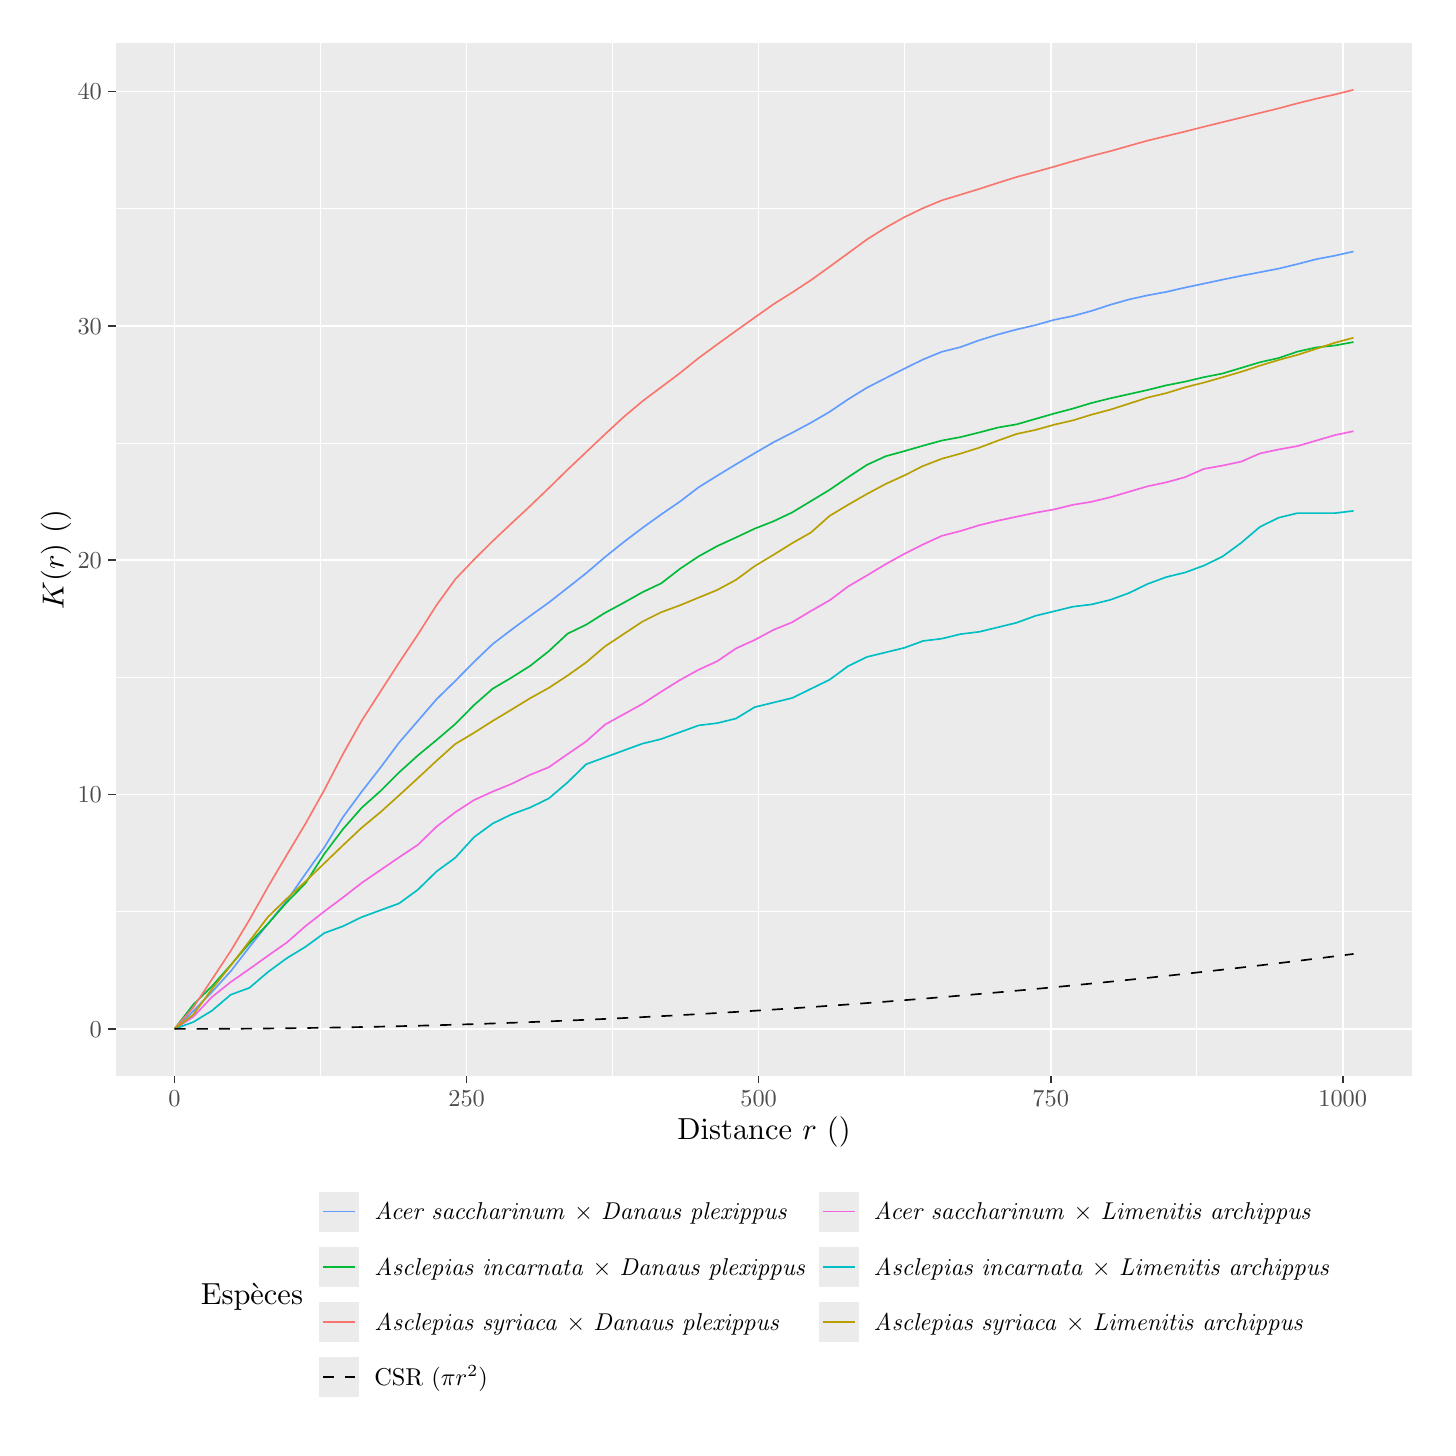
\begin{tikzpicture}[x=1pt,y=1pt]
\definecolor{fillColor}{RGB}{255,255,255}
\path[use as bounding box,fill=fillColor,fill opacity=0.00] (0,0) rectangle (505.89,505.89);
\begin{scope}
\path[clip] (  0.00,  0.00) rectangle (505.89,505.89);
\definecolor{drawColor}{RGB}{255,255,255}
\definecolor{fillColor}{RGB}{255,255,255}

\path[draw=drawColor,line width= 0.6pt,line join=round,line cap=round,fill=fillColor] (  0.00,  0.00) rectangle (505.89,505.89);
\end{scope}
\begin{scope}
\path[clip] ( 31.78,127.12) rectangle (500.39,500.39);
\definecolor{fillColor}{gray}{0.92}

\path[fill=fillColor] ( 31.78,127.12) rectangle (500.39,500.39);
\definecolor{drawColor}{RGB}{255,255,255}

\path[draw=drawColor,line width= 0.3pt,line join=round] ( 31.78,186.42) --
	(500.39,186.42);

\path[draw=drawColor,line width= 0.3pt,line join=round] ( 31.78,271.10) --
	(500.39,271.10);

\path[draw=drawColor,line width= 0.3pt,line join=round] ( 31.78,355.77) --
	(500.39,355.77);

\path[draw=drawColor,line width= 0.3pt,line join=round] ( 31.78,440.44) --
	(500.39,440.44);

\path[draw=drawColor,line width= 0.3pt,line join=round] (105.84,127.12) --
	(105.84,500.39);

\path[draw=drawColor,line width= 0.3pt,line join=round] (211.37,127.12) --
	(211.37,500.39);

\path[draw=drawColor,line width= 0.3pt,line join=round] (316.90,127.12) --
	(316.90,500.39);

\path[draw=drawColor,line width= 0.3pt,line join=round] (422.43,127.12) --
	(422.43,500.39);

\path[draw=drawColor,line width= 0.6pt,line join=round] ( 31.78,144.09) --
	(500.39,144.09);

\path[draw=drawColor,line width= 0.6pt,line join=round] ( 31.78,228.76) --
	(500.39,228.76);

\path[draw=drawColor,line width= 0.6pt,line join=round] ( 31.78,313.43) --
	(500.39,313.43);

\path[draw=drawColor,line width= 0.6pt,line join=round] ( 31.78,398.11) --
	(500.39,398.11);

\path[draw=drawColor,line width= 0.6pt,line join=round] ( 31.78,482.78) --
	(500.39,482.78);

\path[draw=drawColor,line width= 0.6pt,line join=round] ( 53.08,127.12) --
	( 53.08,500.39);

\path[draw=drawColor,line width= 0.6pt,line join=round] (158.61,127.12) --
	(158.61,500.39);

\path[draw=drawColor,line width= 0.6pt,line join=round] (264.14,127.12) --
	(264.14,500.39);

\path[draw=drawColor,line width= 0.6pt,line join=round] (369.66,127.12) --
	(369.66,500.39);

\path[draw=drawColor,line width= 0.6pt,line join=round] (475.19,127.12) --
	(475.19,500.39);
\definecolor{drawColor}{RGB}{97,156,255}

\path[draw=drawColor,line width= 0.6pt,line join=round] ( 53.08,144.09) --
	( 59.84,150.53) --
	( 66.60,157.48) --
	( 73.37,164.92) --
	( 80.13,173.68) --
	( 86.89,182.16) --
	( 93.65,190.46) --
	(100.41,200.16) --
	(107.18,209.68) --
	(113.94,220.64) --
	(120.70,229.82) --
	(127.46,238.51) --
	(134.22,247.55) --
	(140.99,255.38) --
	(147.75,263.22) --
	(154.51,269.82) --
	(161.27,276.68) --
	(168.03,283.16) --
	(174.80,288.32) --
	(181.56,293.32) --
	(188.32,298.16) --
	(195.08,303.46) --
	(201.84,308.79) --
	(208.61,314.58) --
	(215.37,320.00) --
	(222.13,325.12) --
	(228.89,329.97) --
	(235.66,334.62) --
	(242.42,339.79) --
	(249.18,344.00) --
	(255.94,348.10) --
	(262.70,352.12) --
	(269.47,356.06) --
	(276.23,359.50) --
	(282.99,363.12) --
	(289.75,367.05) --
	(296.51,371.63) --
	(303.28,375.80) --
	(310.04,379.26) --
	(316.80,382.67) --
	(323.56,386.00) --
	(330.32,388.77) --
	(337.09,390.46) --
	(343.85,392.94) --
	(350.61,395.02) --
	(357.37,396.83) --
	(364.13,398.39) --
	(370.90,400.31) --
	(377.66,401.69) --
	(384.42,403.54) --
	(391.18,405.75) --
	(397.94,407.67) --
	(404.71,409.17) --
	(411.47,410.41) --
	(418.23,411.97) --
	(424.99,413.39) --
	(431.76,414.84) --
	(438.52,416.22) --
	(445.28,417.52) --
	(452.04,418.82) --
	(458.80,420.45) --
	(465.57,422.21) --
	(472.33,423.49) --
	(479.09,425.01);
\definecolor{drawColor}{RGB}{245,100,227}

\path[draw=drawColor,line width= 0.6pt,line join=round] ( 53.08,144.09) --
	( 59.84,148.48) --
	( 66.60,155.63) --
	( 73.37,161.02) --
	( 80.13,165.75) --
	( 86.89,170.58) --
	( 93.65,175.31) --
	(100.41,181.25) --
	(107.18,186.53) --
	(113.94,191.59) --
	(120.70,196.86) --
	(127.46,201.48) --
	(134.22,206.10) --
	(140.99,210.61) --
	(147.75,217.20) --
	(154.51,222.37) --
	(161.27,226.77) --
	(168.03,229.85) --
	(174.80,232.60) --
	(181.56,235.90) --
	(188.32,238.65) --
	(195.08,243.37) --
	(201.84,247.99) --
	(208.61,254.04) --
	(215.37,257.78) --
	(222.13,261.52) --
	(228.89,265.91) --
	(235.66,270.13) --
	(242.42,273.87) --
	(249.18,276.95) --
	(255.94,281.56) --
	(262.70,284.64) --
	(269.47,288.27) --
	(276.23,291.02) --
	(282.99,295.09) --
	(289.75,298.94) --
	(296.51,303.99) --
	(303.28,307.95) --
	(310.04,312.02) --
	(316.80,315.76) --
	(323.56,319.17) --
	(330.32,322.25) --
	(337.09,324.01) --
	(343.85,326.10) --
	(350.61,327.74) --
	(357.37,329.17) --
	(364.13,330.60) --
	(370.90,331.81) --
	(377.66,333.46) --
	(384.42,334.56) --
	(391.18,336.21) --
	(397.94,338.19) --
	(404.71,340.17) --
	(411.47,341.60) --
	(418.23,343.47) --
	(424.99,346.44) --
	(431.76,347.65) --
	(438.52,349.08) --
	(445.28,352.04) --
	(452.04,353.47) --
	(458.80,354.68) --
	(465.57,356.66) --
	(472.33,358.65) --
	(479.09,360.07);
\definecolor{drawColor}{RGB}{0,186,56}

\path[draw=drawColor,line width= 0.6pt,line join=round] ( 53.08,144.09) --
	( 59.84,152.87) --
	( 66.60,159.52) --
	( 73.37,167.15) --
	( 80.13,175.04) --
	( 86.89,182.14) --
	( 93.65,189.85) --
	(100.41,196.77) --
	(107.18,207.33) --
	(113.94,216.29) --
	(120.70,224.00) --
	(127.46,230.03) --
	(134.22,236.78) --
	(140.99,242.90) --
	(147.75,248.48) --
	(154.51,254.25) --
	(161.27,261.08) --
	(168.03,267.02) --
	(174.80,271.01) --
	(181.56,275.27) --
	(188.32,280.59) --
	(195.08,286.89) --
	(201.84,290.17) --
	(208.61,294.43) --
	(215.37,298.07) --
	(222.13,301.88) --
	(228.89,305.07) --
	(235.66,310.31) --
	(242.42,314.83) --
	(249.18,318.56) --
	(255.94,321.66) --
	(262.70,324.85) --
	(269.47,327.51) --
	(276.23,330.71) --
	(282.99,334.79) --
	(289.75,338.87) --
	(296.51,343.48) --
	(303.28,347.91) --
	(310.04,351.02) --
	(316.80,352.88) --
	(323.56,354.83) --
	(330.32,356.70) --
	(337.09,357.94) --
	(343.85,359.62) --
	(350.61,361.40) --
	(357.37,362.55) --
	(364.13,364.50) --
	(370.90,366.45) --
	(377.66,368.23) --
	(384.42,370.27) --
	(391.18,371.95) --
	(397.94,373.46) --
	(404.71,374.97) --
	(411.47,376.65) --
	(418.23,377.98) --
	(424.99,379.58) --
	(431.76,380.91) --
	(438.52,382.95) --
	(445.28,384.99) --
	(452.04,386.50) --
	(458.80,388.82) --
	(465.57,390.33) --
	(472.33,391.04) --
	(479.09,392.28);
\definecolor{drawColor}{RGB}{0,191,196}

\path[draw=drawColor,line width= 0.6pt,line join=round] ( 53.08,144.09) --
	( 59.84,146.56) --
	( 66.60,150.68) --
	( 73.37,156.45) --
	( 80.13,158.93) --
	( 86.89,164.70) --
	( 93.65,169.65) --
	(100.41,173.77) --
	(107.18,178.72) --
	(113.94,181.19) --
	(120.70,184.49) --
	(127.46,186.97) --
	(134.22,189.44) --
	(140.99,194.39) --
	(147.75,200.99) --
	(154.51,205.93) --
	(161.27,213.36) --
	(168.03,218.30) --
	(174.80,221.60) --
	(181.56,224.08) --
	(188.32,227.38) --
	(195.08,233.15) --
	(201.84,239.75) --
	(208.61,242.22) --
	(215.37,244.69) --
	(222.13,247.17) --
	(228.89,248.82) --
	(235.66,251.29) --
	(242.42,253.76) --
	(249.18,254.59) --
	(255.94,256.24) --
	(262.70,260.36) --
	(269.47,262.01) --
	(276.23,263.66) --
	(282.99,266.96) --
	(289.75,270.26) --
	(296.51,275.21) --
	(303.28,278.50) --
	(310.04,280.15) --
	(316.80,281.80) --
	(323.56,284.28) --
	(330.32,285.10) --
	(337.09,286.75) --
	(343.85,287.58) --
	(350.61,289.22) --
	(357.37,290.87) --
	(364.13,293.35) --
	(370.90,295.00) --
	(377.66,296.65) --
	(384.42,297.47) --
	(391.18,299.12) --
	(397.94,301.59) --
	(404.71,304.89) --
	(411.47,307.37) --
	(418.23,309.02) --
	(424.99,311.49) --
	(431.76,314.79) --
	(438.52,319.74) --
	(445.28,325.51) --
	(452.04,328.81) --
	(458.80,330.46) --
	(465.57,330.46) --
	(472.33,330.46) --
	(479.09,331.28);
\definecolor{drawColor}{RGB}{248,118,109}

\path[draw=drawColor,line width= 0.6pt,line join=round] ( 53.08,144.09) --
	( 59.84,151.86) --
	( 66.60,161.99) --
	( 73.37,172.26) --
	( 80.13,183.51) --
	( 86.89,195.52) --
	( 93.65,206.98) --
	(100.41,218.29) --
	(107.18,230.40) --
	(113.94,243.43) --
	(120.70,255.45) --
	(127.46,265.96) --
	(134.22,276.45) --
	(140.99,286.59) --
	(147.75,297.24) --
	(154.51,306.56) --
	(161.27,313.67) --
	(168.03,320.37) --
	(174.80,326.74) --
	(181.56,333.03) --
	(188.32,339.53) --
	(195.08,346.15) --
	(201.84,352.55) --
	(208.61,358.96) --
	(215.37,365.21) --
	(222.13,370.89) --
	(228.89,375.95) --
	(235.66,381.05) --
	(242.42,386.48) --
	(249.18,391.45) --
	(255.94,396.34) --
	(262.70,401.14) --
	(269.47,405.94) --
	(276.23,410.19) --
	(282.99,414.62) --
	(289.75,419.48) --
	(296.51,424.41) --
	(303.28,429.37) --
	(310.04,433.61) --
	(316.80,437.41) --
	(323.56,440.67) --
	(330.32,443.48) --
	(337.09,445.54) --
	(343.85,447.61) --
	(350.61,449.81) --
	(357.37,451.93) --
	(364.13,453.76) --
	(370.90,455.65) --
	(377.66,457.62) --
	(384.42,459.52) --
	(391.18,461.26) --
	(397.94,463.18) --
	(404.71,465.08) --
	(411.47,466.72) --
	(418.23,468.36) --
	(424.99,470.07) --
	(431.76,471.74) --
	(438.52,473.38) --
	(445.28,475.07) --
	(452.04,476.73) --
	(458.80,478.53) --
	(465.57,480.21) --
	(472.33,481.74) --
	(479.09,483.42);
\definecolor{drawColor}{RGB}{183,159,0}

\path[draw=drawColor,line width= 0.6pt,line join=round] ( 53.08,144.09) --
	( 59.84,149.27) --
	( 66.60,158.52) --
	( 73.37,166.99) --
	( 80.13,175.80) --
	( 86.89,184.62) --
	( 93.65,191.19) --
	(100.41,197.39) --
	(107.18,203.94) --
	(113.94,210.44) --
	(120.70,216.79) --
	(127.46,222.39) --
	(134.22,228.50) --
	(140.99,234.70) --
	(147.75,240.99) --
	(154.51,247.04) --
	(161.27,251.08) --
	(168.03,255.38) --
	(174.80,259.44) --
	(181.56,263.57) --
	(188.32,267.33) --
	(195.08,271.76) --
	(201.84,276.56) --
	(208.61,282.32) --
	(215.37,286.78) --
	(222.13,291.27) --
	(228.89,294.65) --
	(235.66,297.14) --
	(242.42,299.93) --
	(249.18,302.70) --
	(255.94,306.35) --
	(262.70,311.32) --
	(269.47,315.38) --
	(276.23,319.59) --
	(282.99,323.44) --
	(289.75,329.45) --
	(296.51,333.51) --
	(303.28,337.40) --
	(310.04,341.01) --
	(316.80,344.10) --
	(323.56,347.51) --
	(330.32,350.12) --
	(337.09,351.98) --
	(343.85,354.12) --
	(350.61,356.67) --
	(357.37,359.09) --
	(364.13,360.52) --
	(370.90,362.42) --
	(377.66,363.97) --
	(384.42,366.05) --
	(391.18,367.85) --
	(397.94,370.01) --
	(404.71,372.23) --
	(411.47,373.83) --
	(418.23,375.93) --
	(424.99,377.63) --
	(431.76,379.56) --
	(438.52,381.54) --
	(445.28,383.77) --
	(452.04,385.80) --
	(458.80,387.64) --
	(465.57,389.82) --
	(472.33,392.03) --
	(479.09,393.84);
\definecolor{drawColor}{RGB}{0,0,0}

\path[draw=drawColor,line width= 0.6pt,dash pattern=on 4pt off 4pt ,line join=round] ( 53.08,144.09) --
	( 59.84,144.09) --
	( 66.60,144.11) --
	( 73.37,144.15) --
	( 80.13,144.19) --
	( 86.89,144.26) --
	( 93.65,144.33) --
	(100.41,144.42) --
	(107.18,144.52) --
	(113.94,144.64) --
	(120.70,144.77) --
	(127.46,144.91) --
	(134.22,145.07) --
	(140.99,145.24) --
	(147.75,145.42) --
	(154.51,145.62) --
	(161.27,145.83) --
	(168.03,146.06) --
	(174.80,146.30) --
	(181.56,146.55) --
	(188.32,146.82) --
	(195.08,147.10) --
	(201.84,147.39) --
	(208.61,147.70) --
	(215.37,148.02) --
	(222.13,148.35) --
	(228.89,148.70) --
	(235.66,149.06) --
	(242.42,149.44) --
	(249.18,149.83) --
	(255.94,150.23) --
	(262.70,150.65) --
	(269.47,151.08) --
	(276.23,151.52) --
	(282.99,151.98) --
	(289.75,152.45) --
	(296.51,152.93) --
	(303.28,153.43) --
	(310.04,153.94) --
	(316.80,154.47) --
	(323.56,155.01) --
	(330.32,155.56) --
	(337.09,156.13) --
	(343.85,156.71) --
	(350.61,157.30) --
	(357.37,157.91) --
	(364.13,158.53) --
	(370.90,159.16) --
	(377.66,159.81) --
	(384.42,160.48) --
	(391.18,161.15) --
	(397.94,161.84) --
	(404.71,162.54) --
	(411.47,163.26) --
	(418.23,163.99) --
	(424.99,164.74) --
	(431.76,165.49) --
	(438.52,166.26) --
	(445.28,167.05) --
	(452.04,167.85) --
	(458.80,168.66) --
	(465.57,169.49) --
	(472.33,170.33) --
	(479.09,171.18);
\end{scope}
\begin{scope}
\path[clip] (  0.00,  0.00) rectangle (505.89,505.89);
\definecolor{drawColor}{gray}{0.30}

\node[text=drawColor,anchor=base east,inner sep=0pt, outer sep=0pt, scale=  0.88] at ( 26.83,141.08) {0};

\node[text=drawColor,anchor=base east,inner sep=0pt, outer sep=0pt, scale=  0.88] at ( 26.83,225.75) {10};

\node[text=drawColor,anchor=base east,inner sep=0pt, outer sep=0pt, scale=  0.88] at ( 26.83,310.43) {20};

\node[text=drawColor,anchor=base east,inner sep=0pt, outer sep=0pt, scale=  0.88] at ( 26.83,395.10) {30};

\node[text=drawColor,anchor=base east,inner sep=0pt, outer sep=0pt, scale=  0.88] at ( 26.83,479.78) {40};
\end{scope}
\begin{scope}
\path[clip] (  0.00,  0.00) rectangle (505.89,505.89);
\definecolor{drawColor}{gray}{0.20}

\path[draw=drawColor,line width= 0.6pt,line join=round] ( 29.03,144.09) --
	( 31.78,144.09);

\path[draw=drawColor,line width= 0.6pt,line join=round] ( 29.03,228.76) --
	( 31.78,228.76);

\path[draw=drawColor,line width= 0.6pt,line join=round] ( 29.03,313.43) --
	( 31.78,313.43);

\path[draw=drawColor,line width= 0.6pt,line join=round] ( 29.03,398.11) --
	( 31.78,398.11);

\path[draw=drawColor,line width= 0.6pt,line join=round] ( 29.03,482.78) --
	( 31.78,482.78);
\end{scope}
\begin{scope}
\path[clip] (  0.00,  0.00) rectangle (505.89,505.89);
\definecolor{drawColor}{gray}{0.20}

\path[draw=drawColor,line width= 0.6pt,line join=round] ( 53.08,124.37) --
	( 53.08,127.12);

\path[draw=drawColor,line width= 0.6pt,line join=round] (158.61,124.37) --
	(158.61,127.12);

\path[draw=drawColor,line width= 0.6pt,line join=round] (264.14,124.37) --
	(264.14,127.12);

\path[draw=drawColor,line width= 0.6pt,line join=round] (369.66,124.37) --
	(369.66,127.12);

\path[draw=drawColor,line width= 0.6pt,line join=round] (475.19,124.37) --
	(475.19,127.12);
\end{scope}
\begin{scope}
\path[clip] (  0.00,  0.00) rectangle (505.89,505.89);
\definecolor{drawColor}{gray}{0.30}

\node[text=drawColor,anchor=base,inner sep=0pt, outer sep=0pt, scale=  0.88] at ( 53.08,116.16) {0};

\node[text=drawColor,anchor=base,inner sep=0pt, outer sep=0pt, scale=  0.88] at (158.61,116.16) {250};

\node[text=drawColor,anchor=base,inner sep=0pt, outer sep=0pt, scale=  0.88] at (264.14,116.16) {500};

\node[text=drawColor,anchor=base,inner sep=0pt, outer sep=0pt, scale=  0.88] at (369.66,116.16) {750};

\node[text=drawColor,anchor=base,inner sep=0pt, outer sep=0pt, scale=  0.88] at (475.19,116.16) {1000};
\end{scope}
\begin{scope}
\path[clip] (  0.00,  0.00) rectangle (505.89,505.89);
\definecolor{drawColor}{RGB}{0,0,0}

\node[text=drawColor,anchor=base,inner sep=0pt, outer sep=0pt, scale=  1.10] at (266.08,104.08) {Distance $r$ (\unit{\m})};
\end{scope}
\begin{scope}
\path[clip] (  0.00,  0.00) rectangle (505.89,505.89);
\definecolor{drawColor}{RGB}{0,0,0}

\node[text=drawColor,rotate= 90.00,anchor=base,inner sep=0pt, outer sep=0pt, scale=  1.10] at ( 13.01,313.75) {$K(r)$ (\unit{\km\squared})};
\end{scope}
\begin{scope}
\path[clip] (  0.00,  0.00) rectangle (505.89,505.89);
\definecolor{fillColor}{RGB}{255,255,255}

\path[fill=fillColor] ( 57.06,  5.50) rectangle (475.11, 90.82);
\end{scope}
\begin{scope}
\path[clip] (  0.00,  0.00) rectangle (505.89,505.89);
\definecolor{drawColor}{RGB}{0,0,0}

\node[text=drawColor,anchor=base west,inner sep=0pt, outer sep=0pt, scale=  1.10] at ( 62.56, 44.40) {Espèces};
\end{scope}
\begin{scope}
\path[clip] (  0.00,  0.00) rectangle (505.89,505.89);
\definecolor{fillColor}{gray}{0.92}

\path[fill=fillColor] (105.29, 70.86) rectangle (119.75, 85.32);
\definecolor{drawColor}{RGB}{97,156,255}

\path[draw=drawColor,line width= 0.6pt,line join=round] (106.74, 78.09) -- (118.30, 78.09);
\end{scope}
\begin{scope}
\path[clip] (  0.00,  0.00) rectangle (505.89,505.89);
\definecolor{fillColor}{gray}{0.92}

\path[fill=fillColor] (285.78, 70.86) rectangle (300.23, 85.32);
\definecolor{drawColor}{RGB}{245,100,227}

\path[draw=drawColor,line width= 0.6pt,line join=round] (287.22, 78.09) -- (298.78, 78.09);
\end{scope}
\begin{scope}
\path[clip] (  0.00,  0.00) rectangle (505.89,505.89);
\definecolor{fillColor}{gray}{0.92}

\path[fill=fillColor] (105.29, 50.91) rectangle (119.75, 65.36);
\definecolor{drawColor}{RGB}{0,186,56}

\path[draw=drawColor,line width= 0.6pt,line join=round] (106.74, 58.14) -- (118.30, 58.14);
\end{scope}
\begin{scope}
\path[clip] (  0.00,  0.00) rectangle (505.89,505.89);
\definecolor{fillColor}{gray}{0.92}

\path[fill=fillColor] (285.78, 50.91) rectangle (300.23, 65.36);
\definecolor{drawColor}{RGB}{0,191,196}

\path[draw=drawColor,line width= 0.6pt,line join=round] (287.22, 58.14) -- (298.78, 58.14);
\end{scope}
\begin{scope}
\path[clip] (  0.00,  0.00) rectangle (505.89,505.89);
\definecolor{fillColor}{gray}{0.92}

\path[fill=fillColor] (105.29, 30.95) rectangle (119.75, 45.41);
\definecolor{drawColor}{RGB}{248,118,109}

\path[draw=drawColor,line width= 0.6pt,line join=round] (106.74, 38.18) -- (118.30, 38.18);
\end{scope}
\begin{scope}
\path[clip] (  0.00,  0.00) rectangle (505.89,505.89);
\definecolor{fillColor}{gray}{0.92}

\path[fill=fillColor] (285.78, 30.95) rectangle (300.23, 45.41);
\definecolor{drawColor}{RGB}{183,159,0}

\path[draw=drawColor,line width= 0.6pt,line join=round] (287.22, 38.18) -- (298.78, 38.18);
\end{scope}
\begin{scope}
\path[clip] (  0.00,  0.00) rectangle (505.89,505.89);
\definecolor{fillColor}{gray}{0.92}

\path[fill=fillColor] (105.29, 11.00) rectangle (119.75, 25.45);
\definecolor{drawColor}{RGB}{0,0,0}

\path[draw=drawColor,line width= 0.6pt,dash pattern=on 4pt off 4pt ,line join=round] (106.74, 18.23) -- (118.30, 18.23);
\end{scope}
\begin{scope}
\path[clip] (  0.00,  0.00) rectangle (505.89,505.89);
\definecolor{drawColor}{RGB}{0,0,0}

\node[text=drawColor,anchor=base west,inner sep=0pt, outer sep=0pt, scale=  0.88] at (125.25, 75.08) {\textit{Acer saccharinum} $\times$ \textit{Danaus plexippus}};
\end{scope}
\begin{scope}
\path[clip] (  0.00,  0.00) rectangle (505.89,505.89);
\definecolor{drawColor}{RGB}{0,0,0}

\node[text=drawColor,anchor=base west,inner sep=0pt, outer sep=0pt, scale=  0.88] at (305.73, 75.08) {\textit{Acer saccharinum} $\times$ \textit{Limenitis archippus}};
\end{scope}
\begin{scope}
\path[clip] (  0.00,  0.00) rectangle (505.89,505.89);
\definecolor{drawColor}{RGB}{0,0,0}

\node[text=drawColor,anchor=base west,inner sep=0pt, outer sep=0pt, scale=  0.88] at (125.25, 55.13) {\textit{Asclepias incarnata} $\times$ \textit{Danaus plexippus}};
\end{scope}
\begin{scope}
\path[clip] (  0.00,  0.00) rectangle (505.89,505.89);
\definecolor{drawColor}{RGB}{0,0,0}

\node[text=drawColor,anchor=base west,inner sep=0pt, outer sep=0pt, scale=  0.88] at (305.73, 55.13) {\textit{Asclepias incarnata} $\times$ \textit{Limenitis archippus}};
\end{scope}
\begin{scope}
\path[clip] (  0.00,  0.00) rectangle (505.89,505.89);
\definecolor{drawColor}{RGB}{0,0,0}

\node[text=drawColor,anchor=base west,inner sep=0pt, outer sep=0pt, scale=  0.88] at (125.25, 35.18) {\textit{Asclepias syriaca} $\times$ \textit{Danaus plexippus}};
\end{scope}
\begin{scope}
\path[clip] (  0.00,  0.00) rectangle (505.89,505.89);
\definecolor{drawColor}{RGB}{0,0,0}

\node[text=drawColor,anchor=base west,inner sep=0pt, outer sep=0pt, scale=  0.88] at (305.73, 35.18) {\textit{Asclepias syriaca} $\times$ \textit{Limenitis archippus}};
\end{scope}
\begin{scope}
\path[clip] (  0.00,  0.00) rectangle (505.89,505.89);
\definecolor{drawColor}{RGB}{0,0,0}

\node[text=drawColor,anchor=base west,inner sep=0pt, outer sep=0pt, scale=  0.88] at (125.25, 15.22) {CSR ($\pi r^2$)};
\end{scope}
\end{tikzpicture}
